\documentclass[12pt,a4paper,titlepage]{article}
\usepackage[utf8]{inputenc}
\usepackage[russian]{babel}
\usepackage[OT1]{fontenc}
\usepackage{amsmath}
\usepackage{amsfonts}
\usepackage{amssymb}
\usepackage{graphicx}
\author{Н.Е.Богданов}
\title{ « Параллельные вычисления »}
\frenchspacing
\begin{document}
\maketitle
\tableofcontents
\newpage
\section{Задание}

\begin{enumerate}
\item 
Постановка задачи
\begin{itemize}
\item 
Описание назначения проектируемой системы
\item 
Функциональные требования (текстовое описание Участников и их Интересов)
\item
Описание бизнес-процессов (этапы, Участники)
\end{itemize} 
\item
Разработка вариантов использования (обобщенная диаграмма(ы) прецедентов для всех ролей)
\item
Подробное описание всех вариантов использования (текстовое описание с альтернативами)
\item
Разработка статической объектной модели предметной области (диаграмма классов)
\item
Разработка динамической объектной модели предметной области (диаграмма последовательности)
\item
Проектирование слоя бизнес-логики (выбор архитектурного шаблона уровня бизнес-логики)
\item
Реализация слоя бизнес-логики (Java, NetBeans), unit-тестирование (JUnit), вместо слоя хранения - шаблон "Репозиторий"
\item
Проектирование слоя источников данных (выбор архитектурного шаблона уровня доступа к данным: DB + внешний сервис)
\item
Реализация слоя источников данных (JavaDB, NetBeans), unit-тестирование
\item
Проектирование сервисного слоя и слоя представления: GUI (Swing), внешний сервис
\item
Реализация слоев представления, сервисного слоя, unit-тестирование сервисного слоя
\item
Комплексное тестирование системы
\item
Пояснительная записка (включает все разделы, указанные выше, а также выводы)
\end{enumerate}
\section{Решение}
\subsection{Постановка задачи}
Заказ услуг по строительным работам.
Создание и управления заказами на строительные работы, а так же учёт требуемых ресурсов на складе.
\subsection{Роли}
\begin{itemize}
\item Клиент
\begin{enumerate}
\item Заказывает работу.
\item Принимает результат.
\item Оплачивает работу.
\end{enumerate}
\item Менеджер
\begin{enumerate}
\item Составляет смету + смету доработок (на основе списка доработок от Прораба).
\item Ведёт учёт ресурсов со склада.(дозаказывает по мере надобности).
\item Ведёт учёт бюджета компании.
\item Принимает оплату от клиента.
\end{enumerate}
\item Прораб
\begin{enumerate}
\item Получает список работ.
\item Выполняет работу.
\item Составляет список доработок.
\item Отдаёт работу на приём Клиенту.
\end{enumerate}
\end{itemize}
\newpage
\subsection{Подробное описание вариантов использования}
\begin{enumerate}
\item
Процесс оформления заказа. прописываются все требуемые ресурсы и услуги оказываемые прорабом. Если ресурсов на складе не хватает то происходит дополнительный заказ ресурсов.
\item
Процесс сдачи/приёма работы.

2 Варианта:
\begin{itemize}
\item Первый. Успешная сдача объекта клиент принимает работу прораба и получает смету (составленную менеджером) со списком проведённых работ.
\item Второй. В случае если клиент требует доработки, прораб составляет список требуемых работ и(или) ресурсов), а менеджер составляет смету доработок,после чего клиент оплачивает 85\% от текущего заказа без сметы доработок. а дальше выполняются действия как в первом варианте или повторные доработки.
\end{itemize}
\item
Процесс оплаты счёта. 2 варианта действий, клиент может оплатить:
	\begin{itemize}
		\item наличными или
		\item по безналичному расчёту.
	\end{itemize}
\end{enumerate}
\newpage
\subsection{Use - case диаграмма}
\begin{figure}[!ht]
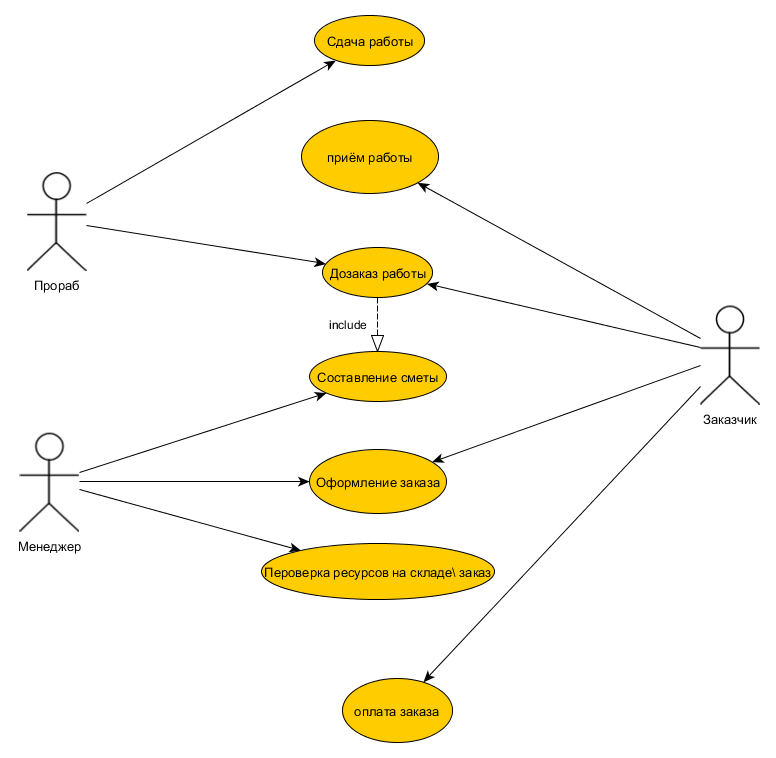
\includegraphics[scale=0.5]{uml_use_case.png}\caption{}
\end{figure}
\newpage
\subsection{Статическая модель предметной области (uml диаграмма классов)} 
\begin{figure}[!ht]
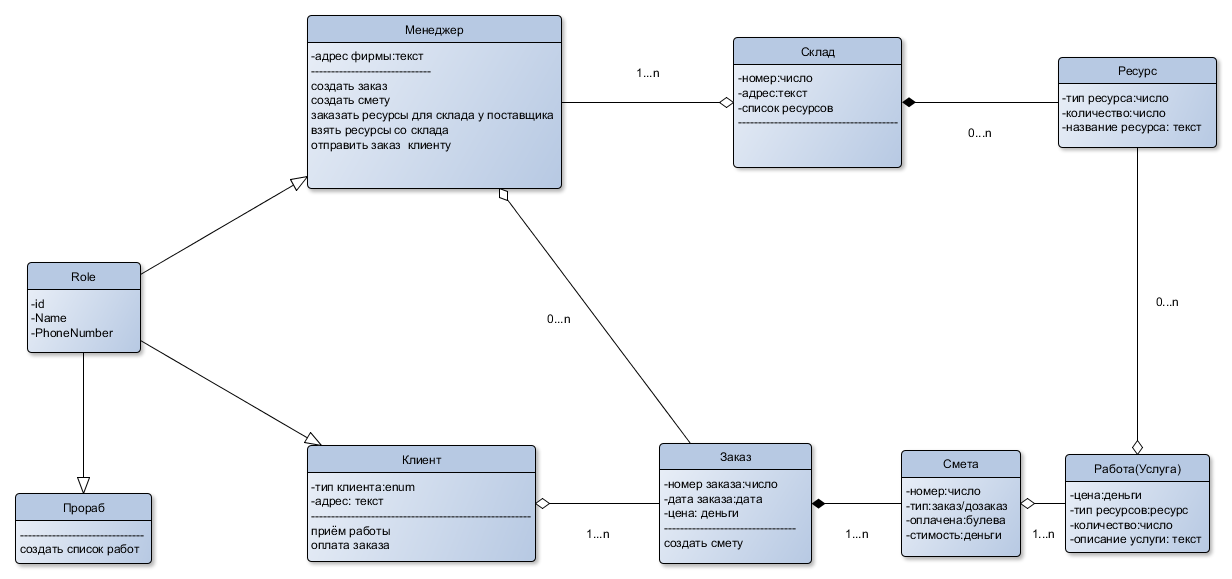
\includegraphics[scale=0.3]{uml_class_diagram.png}\caption{}
\end{figure}
\newpage
\subsection{Диаграмма последовательностей}
\begin{figure}[!ht]
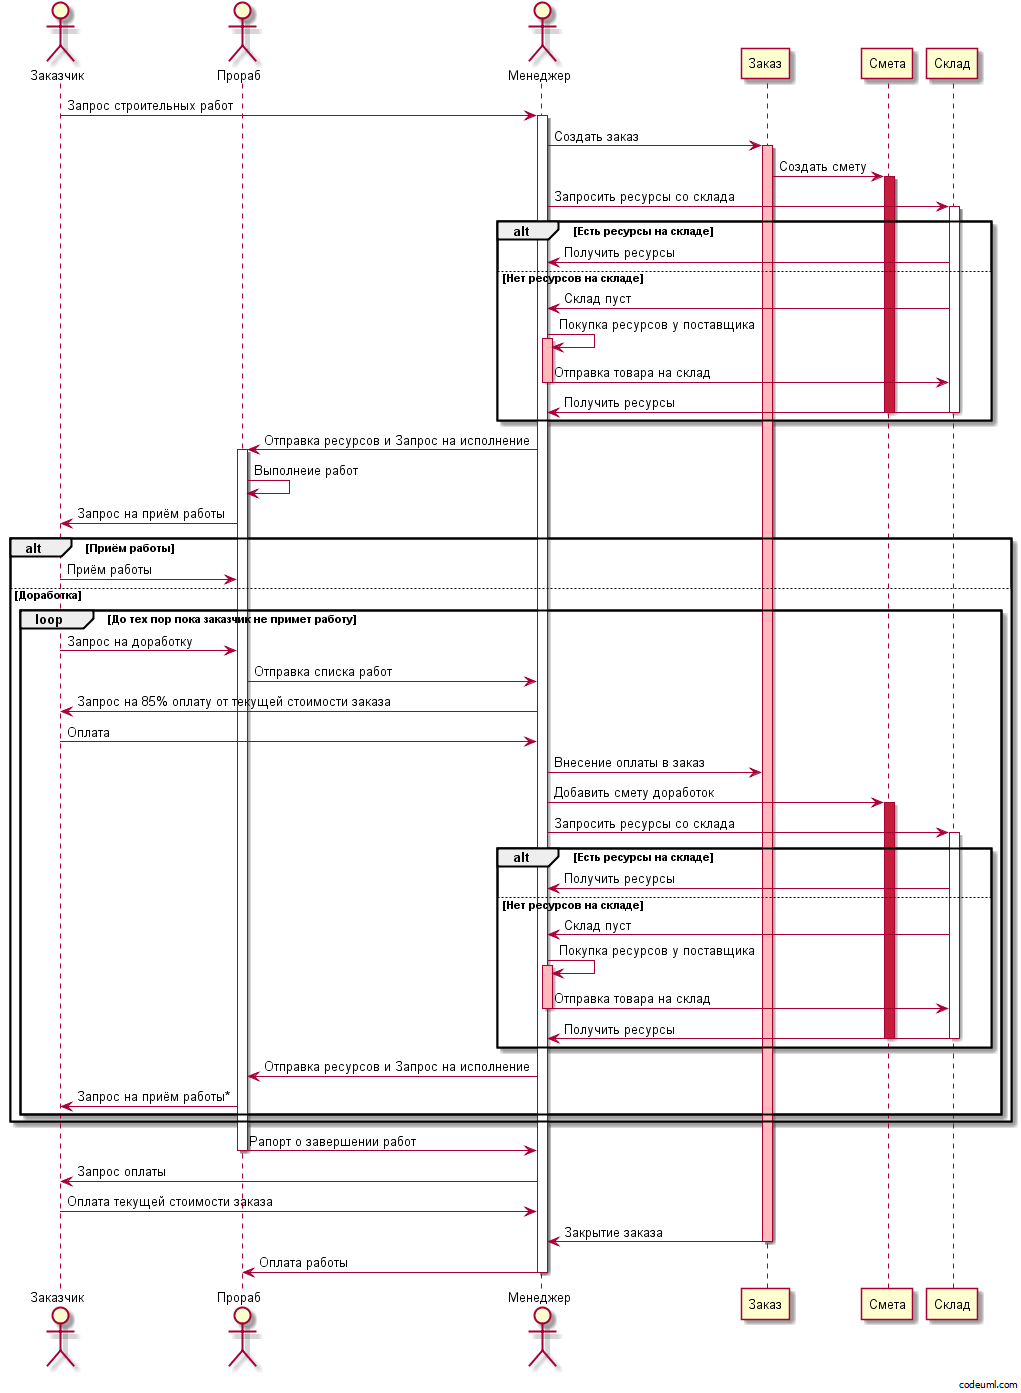
\includegraphics[scale=0.5]{getimage.png}\caption{}
\end{figure}
\newpage
\subsection{Слой бизнес-логики}
В качестве типового решения бизнес-логики была выбрана: 
\\
Модель предметной области(Domain Model).
Классы бизнес логики соответствуют uml диаграмме (рис.2).
\begin{figure}[!ht]
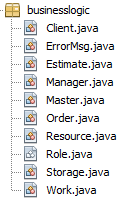
\includegraphics[scale=0.8]{bisnesslogic.png}\caption{}
\end{figure}
\\
\textbf{Сущности объекты с которыми работают роли:}
\begin{itemize}
\item Order - Заказ
\item Estimate - Смета в заказе
\item Storage - Склад содержащий список с ресурсами.
\item Work - Работы содержащие список ресурсов
\item Resource - Ресурсы.
\end{itemize}

\textbf{Роли:}
\begin{itemize}
\item Role - абстрактное представление роли.
\item Manager - Роль менеджера.
\item Client - Роль заказчика
\item Master - Роль прораба
\end{itemize}
Единственный элемент являющийся вспомогательным
ErrorMsg - Содержит код ошибки и сообщение об ошибке
создан специально для обработки ошибок от склада для роли менеджера.
\newpage
\textbf{unit-тестирование (JUnit) бизнес логики:}
\begin{figure}[!ht]
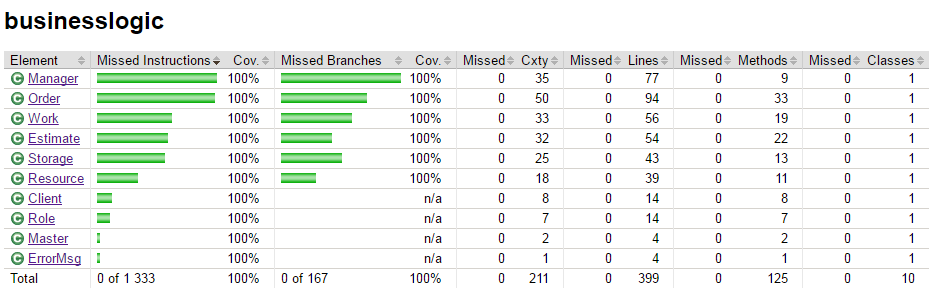
\includegraphics[scale=0.6]{busnesslogicJUintTest.png}\caption{}
\end{figure}
\newpage
\subsection{Слой источников данных}
В качестве решения типового решения
источников данных выбран:
\\
Преобразователь данных \textbf{(Data Mapper)}, также дополнительно для облегчения работы были упрощенна работа с SQL - выражениями по средством добавления паттерна строитель для построения SQL - запросов.(класс QueryBilder),а так - же отделения работы с базой данных в класс DatabaseManager.


Для каждого объекта создан свой Mapper с соответствующей приставкой в названии (пример OrderMapper для объекта Order из слоя бизнес логики) некоторые используют внутри Mapper'ы если объекты составные.
\\
В качестве хранилища данных выбрана СУБД Firebird.
\begin{figure}[!ht]
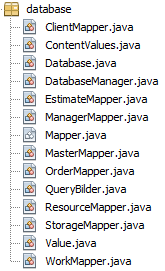
\includegraphics[scale=0.8]{databaseMapper.png}\caption{}
\end{figure}
\newpage
\textbf{Представление таблиц данных в БД.}
\\ 

Таблицы:
\begin{itemize}
\item StorageInformation - информация о складе.
\item Storage - информация о ресурсах на складе и их количество.
\item Resource - информация о ресурсе. 
\item Work - информация о работе.
\item WorksAndResource - информация о ресурсах и их количестве нужном для работы.
\item Estimate - информация о списке смет для заказов.
\item EstimateWorks - информация о списке работ для смет.
\item Manager - инофрмация о менеджерах.
\item Master - информация о прорабах.
\item Client - информация о заказчиках.
\end{itemize}
Дополнительно созданы View для упрощения запросов к данным сущностей бизнес логики распределённым между несколькими таблицами (склады, работы, сметы):
\begin{itemize}
\item StorageView
\item WorkView
\item EstimateView
\end{itemize}
\newpage
\begin{figure}[!ht]
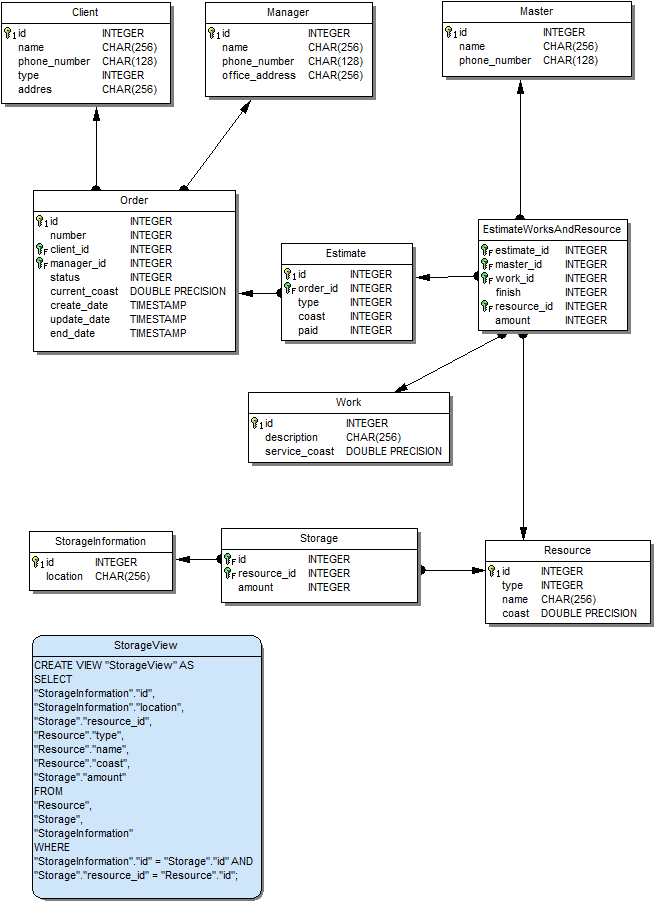
\includegraphics[scale=0.6]{database.png}\caption{}
\end{figure}
\newpage
\textbf{unit-тестирование (JUnit) слоя источников данных:}
\begin{figure}[!ht]
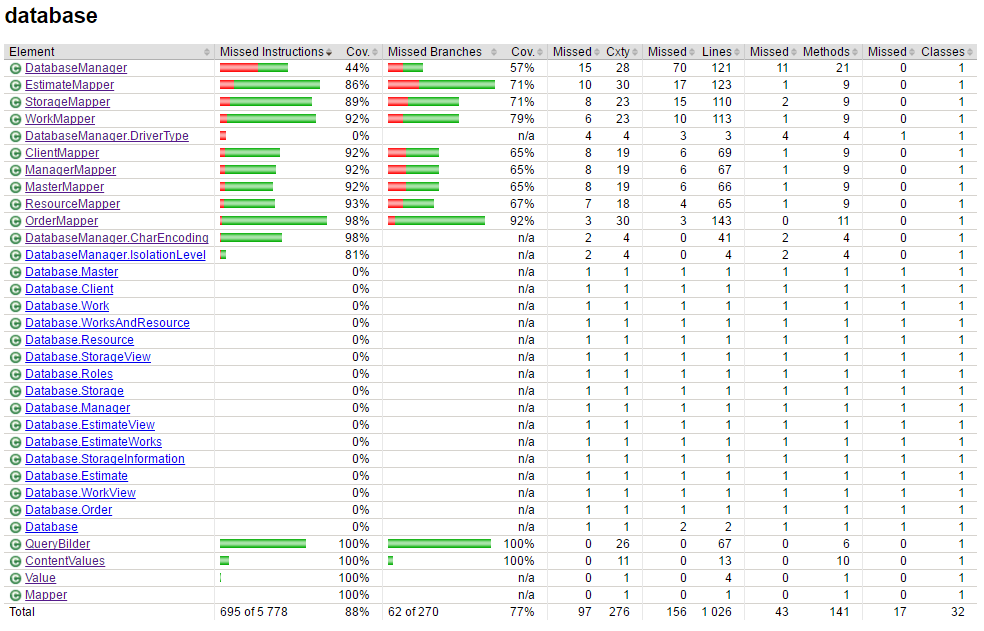
\includegraphics[scale=0.6]{databaseJUnitTest.png}\caption{}
\end{figure}

Не протестированными остались классы содержащие только статические 
имена полей таблиц и названий таблиц в базе данных, а также метод saveArray для нескольких классов, но был позже протестирован при сборке проекта с GUI.
\newpage
\subsection{Сервисный слой и слой представления}
Графика была создана при помощи визуального редактора в NetBeans.
Конифигурационный файл, Swing GUI 

\begin{figure}[!ht]
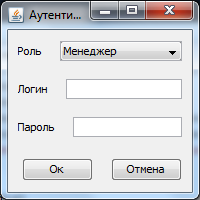
\includegraphics[scale=0.6]{auth.png}\caption{Окно авторизации}
\end{figure}

\begin{figure}[!ht]
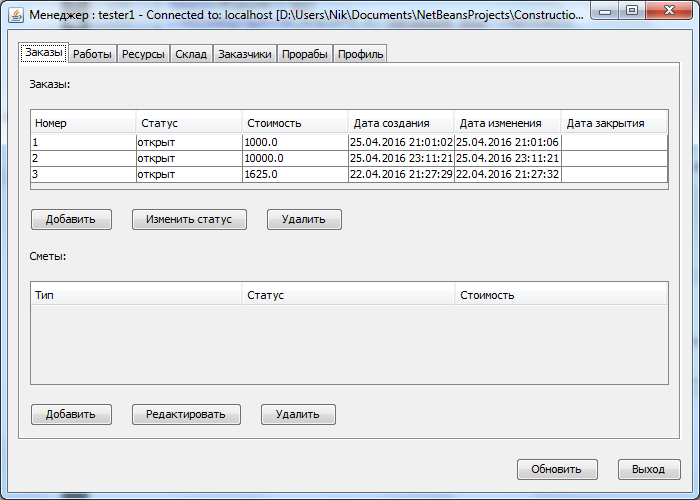
\includegraphics[scale=0.6]{ManagerView.png}\caption{Графическое представление для роли Менеджера}
\end{figure}

\begin{figure}[!ht]
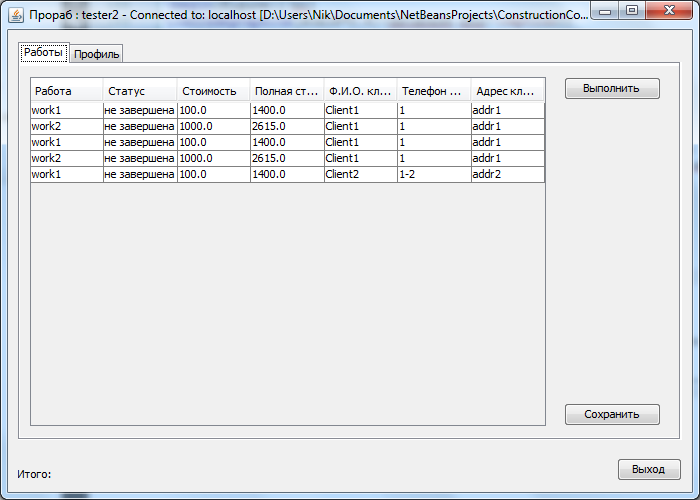
\includegraphics[scale=0.6]{MasterView.png}\caption{Графическое представление для роли Прораба}
\end{figure}

\begin{figure}[!ht]
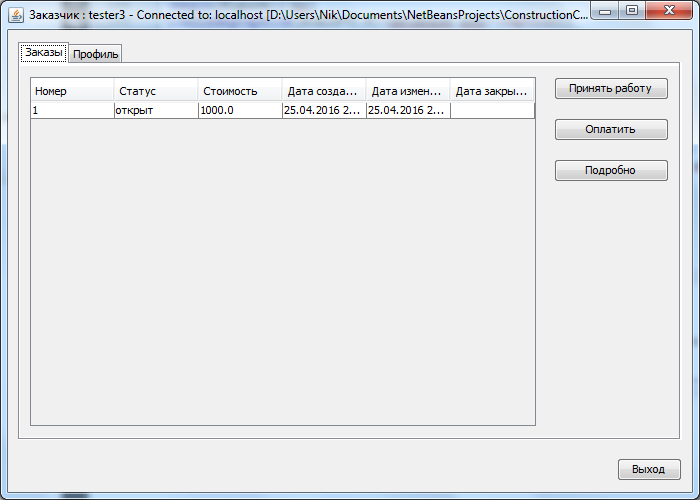
\includegraphics[scale=0.6]{ClientView.png}\caption{Графическое представление для роли Заказчика}
\end{figure}
\newpage
Тестирование графики проводилось полностью при сборке работы всего проекта.
\newpage
\textbf{Тестирование конфигурационного файла:}
\begin{figure}[!ht]
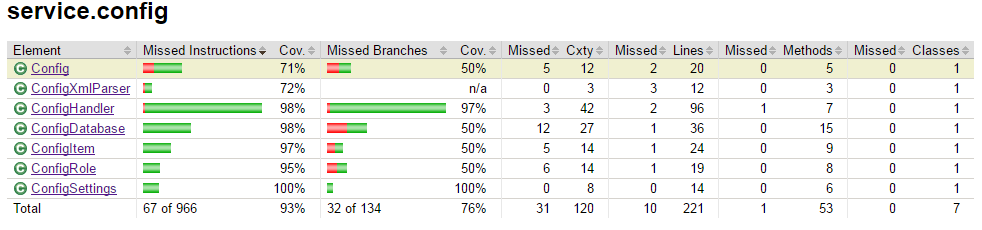
\includegraphics[scale=0.6]{configJUnitTest.png}\caption{}
\end{figure}
\newpage
\section{Заключение}
Данная работа моделирует пример проектирование архитектуры информационной системы для бизнес процессов на примере строительной организации.
\end{document}